%!TEX root = ../thesis.tex
%%--------------------------------------------------------------------------
%% OPENSTACK AND DEVSTACK
%%--------------------------------------------------------------------------


In this chapter we are going to present OpenStack and DevStack; we shall provide a brief overview and focus on the components and aspects that most concern the topics of our thesis.

\section{OpenStack}
\label{sec:openstack}
OpenStack is an open-source cloud computing software platform that provides a complete IaaS solution for public and private clouds. Founded by Nasa\footnote{\url{www.nasa.gov} (2015)} and Rackspace Cloud\footnote{\url{www.rackspace.com} (2015)} in 2010 OpenStack is now one of the biggest open-source projects with more than twenty thousand people working on it and more than twenty million code lines. It is a cloud operating system that controls large pools of compute, storage, and networking resources throughout a datacenter (with the possibility of controlling them trough a dashboard) and enabling enterprises and service providers to offer on-demand computing resources.\\
One of its main strengths is its modularity, which provides the flexibility needed to design different configurations for different cloud environments; its core components are:
\begin{description}
	\item[Compute] The service called \texttt{Nova} is the primary computing engine and it is used to deploy and manage large numbers of Virtual Machines.
	\item[Storage] The storage platform, divided in Object Storage (\texttt{Swift}) and Block Storage (\texttt{Cinder}).
	\item[Network] The service called \texttt{Neutron} offers Networking as a Service
	\item[Dashboard] \texttt{Horizon} that is a dashboard provides users with a graphical user interface to access, provision, and automate cloud-based resources.
	\item[Shared Services] Other services, that makes it easier to manage the IaaS, such as the Identity Service (\texttt{Keystone}), the Image Service (\texttt{Glance}), Telemetry (\texttt{Ceilometer}), Orchestration (\texttt{Heat}) and others.
\end{description}

\begin{figure}[!ht]
\centering{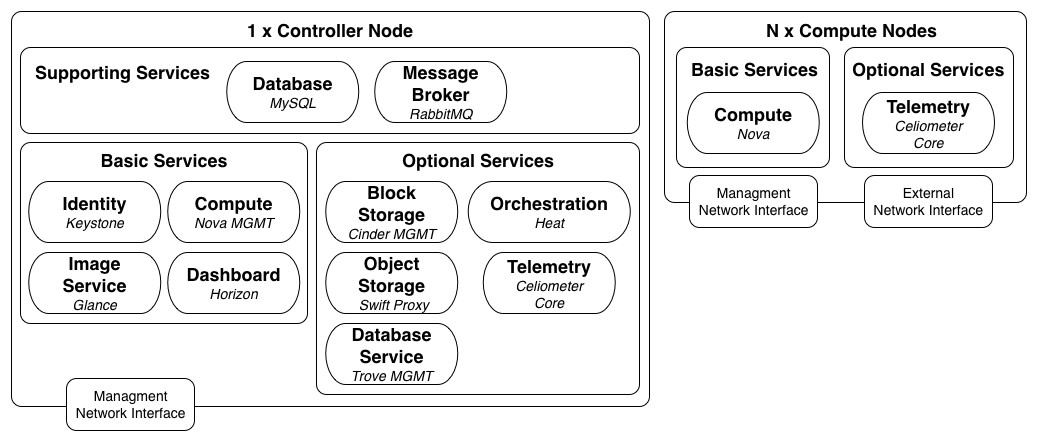
\includegraphics[width=\textwidth]{images/openstack_arch.png}}
\label{fig:openstack_1plusN}
\caption{A ``1 + N'' OpenStack configuration}
\end{figure}

We have decided to focus on the creation of ``1 + N'' installations of OpenStack; these are composed of one \textit{Controller} node and N \textit{Compute} nodes with legacy networking. Legacy networking refers to a basic solution in which we do not deploy \texttt{Neutron} but we exploit \code{nova-network}, a \texttt{Nova} service described in paragraph \ref{par:openstack_nova_net}. The figure~\ref{fig:openstack_1plusN} on page~\pageref{fig:openstack_1plusN} provides a high level view of all the OpenStack services, both basic and optional, that have to be installed both on the Controller and the Compute nodes to setup a ``1 + N'' configuration.\\ 
The Controller node is responsible for globally managing the cloud operations. It runs the user \texttt{Identity} service, the Virtual Machine \texttt{Image} service, the management portion of the \texttt{Compute} service, and a \textit{Dashboard} through which the users can request the creation of new Virtual Machines. Optionally, the node can run the management portions of the \texttt{Block}, \texttt{Object}, and \texttt{Database Storage} services, and the \texttt{Telemetry} and \texttt{Orchestration} services. The Controller node also runs a series of supporting services (i.e., the \texttt{Database} and \texttt{Message Broker} services). Each of the N basic Compute nodes, on the other hand, runs the \texttt{Compute} service and optionally the \texttt{Telemetry} service.

\subsection{Nova}
\label{sec:openstack_nova}
OpenStack Compute module, \texttt{Nova}, is the core of OpenStack; it takes care of deploying and managing Virtual Machines, by placing them on physical machines, letting them communicate, storing their informations on an SQL database, and offering a set of HTTP managed APIs and a command-line client.
In the next paragraphs we will briefly describe the three \texttt{Nova} sub-modules that are relevant for our work.

\subparagraph{Nova-compute}
\label{par:openstack_nova_compute}
The \texttt{nova-compute} is the sub-module that takes care of booting, resizing, live-migrating and destroying the Virtual Machines that are running on the physical servers, and of letting them communicate with the hypervisor.\\
Hereunder are reported four examples of the main commands (also accessible through the Nova APIs) used to boot, resize, destroy and live-migrate Virtual Machines:
\begin{itemize}
	\item \code{\$ nova boot --flavor <flavor> --image <image>}
	\item \code{\$ nova resize --flavor <vm> <flavor>}
	\item \code{\$ nova delete <vm>}
	\item \code{\$ nova live-migration <vm> <host>}
\end{itemize}

\subparagraph{Nova-network}
\label{par:openstack_nova_net}
\texttt{Nova-network} is the basic network management module of OpenStack. It i included directly in \texttt{Nova}. Unlike \texttt{Neutron}, which can virtualize and manage both layer 2 (logical) and layer 3 (network) of the OSI network, \texttt{nova-network} only provides layer 3 virtualization and has some limitations on the network topology.\\
However \texttt{nova-network} is still supported by OpenStack and in powerful enough to support a ``1 + N'' configuration. It also streamlines the installation process as it avoids having to install another service (\texttt{Neutron}) and its dependencies.

\subparagraph{Nova-scheduler}
\label{par:openstack_nova_sched}
\texttt{Nova} uses the \texttt{nova-scheduler} service to determine how to dispatch compute requests. It is used, for example, to determine on which host a Virtual Machine should launch. The system administrator can modify and configure the \code{/etc/nova/nova.conf} configuration file to adjust the criteria under which the \texttt{nova-scheduler} will place the Virtual Machines. The process of placing Virtual Machines on the most suitable host is divided in a \textit{filtering} step, in which a list of candidate hosts is generated, and a \textit{weighing} step in which the list is ordered according to the selected criteria and the best host is chosen.

\subsection{Fake Drivers}
\label{sec:openstack_fake_drivers}
To deal with situations in which the compute nodes are not physical machines that will host real Virtual Machines, but they have be ``fake'' in the sense that they don't host a real hypervisor, OpenStack offers a module called \code{nova.virt.fake} that allows developers, that don't have real hardware, to test \code{Nova} code on compute nodes without a real hypervisor such as \textit{libvirt}. When exploiting this solution Virtual Machines, are mere python objects; in such a way the Virtual Machines are not really spawned but simply stored in the database. However \code{FakeDriver} mimics the correct behavior of a real hypervisor, allowing one to test the rest of the \code{Nova} running flow.\\
This module is not configurable and by default a \code{FakeDriver} offers 1000 VCUs, 800000 MB of RAM, and 600000 GB of Hard Disk. 

\section{DevStack}
\label{sec:devstack}
 
DevStack\footnote{More info at \url{docs.openstack.org/developer/devstack}} is a set of scripts and utilities to quickly deploy an OpenStack cloud environment and it is freely available on GitHub\footnote{\url{github.com/openstack-dev/devstack}}.\\
DevStack allows developers and system administrators to automate the process of installing OpenStack on a server reducing it to a simple command for every installation.\\
The services that are configured by default are Identity (\texttt{Keystone}), Object Storage (\texttt{Swift}), Image Storage (\texttt{Glance}), Block Storage (\texttt{Cinder}), Compute (\texttt{Nova}), Network (\texttt{Nova}), Dashboard (\texttt{Horizon}) and Orchestration (\texttt{Heat}).
The main script is \code{stack.sh}; all the required configurations, such as the Git repositories to use, the services to enable or the OS images to use, can be achieved overriding default environment variables (found in \code{stackrc}) through file \code{local.conf}. This is achieved with a \code{localrc} section, as shown below:
\begin{lstlisting}[numbers=none,label={lst:devstack_local_conf}]
[[local|localrc]]
ADMIN_PASSWORD=secrete
DATABASE_PASSWORD=$ADMIN_PASSWORD
RABBIT_PASSWORD=$ADMIN_PASSWORD
SERVICE_PASSWORD=$ADMIN_PASSWORD
SERVICE_TOKEN=a682f596-76f3-11e3-b3b2-e716f9080d50
# ...
ENABLED_SERVICES=n-cpu,n-api,n-net
# ...
\end{lstlisting}
The environment variable \code{ENABLED\_SERVICES} is used to define the service to run: in listing \ref{lst:devstack_local_conf} the \texttt{Nova} services to install, in a simple compute node installation, are \texttt{nova-compute}, \texttt{nova-api}, \texttt{nova-network}.
By running the script \code{tools/install\_prereqs.sh} it is furthermore possible to install all the dependencies required by the configured services.\\Other useful scripts provided by DevStack are \code{unstack.sh}, that allows to stop everything that was started by \code{stack.sh}, and \code{clean.sh} that tries to remove all the traces left by the OpenStack installation performed by DevStack.
